\section{LSD on the brain.}

The introduction of exogenous entities like LSD or other substances in the organism produces an imbalance with all kinds of consequences.

\subsection{What is a drug?}

Organisms consume different kinds of substances from their environment. Some are assimilated immediately and converted into matter and energy or excrements. We call these food. Others aren't assimilated so easily: because of genetic reasons, copper can accumulate in the liver with severe consequences (Wilson's disease). But other substances, rather than getting accumulated, unchain immense reactions upon the organism. These have a special place in medicine. Because they tend to be similar in structure and/or function to endogenous substances, they can be used to regulate it directly or indirectly.

Many substances can then serve as treatment for many diseases (as insuline does for diabetes). But by their very nature, their presence in high levels can also become toxic: aspirin is for example lethal in about 250 miligrams per kg of body weight (mg / kg). Of course, the lethal thing isn't aspirin itself, but the dose with respect to the measure of body weight. This double action as a remedy and a poison is what the greek word \textit{phármakon} ($\phi\acute{\alpha}\rho\mu\alpha\kappa o\nu$) describes. It was known even back then that the distinction between remedy and poison didn't depend on the substance, but the dosage.

Among the non-foods we find substances that not only act in somatic ways (like potassium cyanide or acetaminophen), but also act upon the nervous system, affecting perception and emotion (thought of as the psychophysiological internal reactions the individual has over important stimuli). These substances are called \textit{drugs}.

It's important to note that the term \enquote{drug} is polysemic, and is sometimes used to denote exclusively substances with effects over the nervous system, whereas other times it's used to refer to any chemical compound used in medicine.

At last, it is important to recognise that many drugs (using the first definition) are illegal and, as such, the term holds another meaning in the scope of law. Historically, humanity's relationship with drugs has been a matter of controversy (see the example with wine in Ancient Rome), and either culturally or systematically their use has been pursued. Around the last third of the 20th century, more strict regulations are put into place in countries like the United States with the \textit{Controlled Substances Act} and \enquote{drug} becomes a term used to designate any substance recognised as such by the Act.

To avoid ambiguity, in this document we'll use the following definitions:

\begin{itemize}
	\item Pharmaceutical: any substance used as treatment for a disease.
	\item Drug: any substance which interacts with the nervous system producing changes in perception and emotion.
\end{itemize}

\subsection{Terminology.}

There is a set of terms associated both to drugs and pharmaceuticals that we define in a quantitative and qualitative way. First, we've got those referring to dosage. Different organisms differ on their particular characteristics and won't react in the same way to the same dose. Because of that, our statements will be statistical and not concrete.

It's common practice to administer a certain dose to a population and observe its effects. The \textit{average effective dose} (ED50) is that which produces the desired effects on 50\% of the individuals it's given to (there may be many different effective doses depending on the desired effects one wishes to induce). The \textit{average lethal dose} (LD50) is that which is enough to end the life of the same percentage of the population. From these two one can extract the margin of safety, which is the ratio of average effective dose to lethal effective dose.

Both pharmaceuticals and drugs lose their effect partially or totally after repeated usage, this phenomenon is known as \textit{tolerance}. Repeated daily doses of aspirin generate a tolerance which makes it much less effective. This capacity for adaptation from the body isn't the same for all substances, so the tolerance induced by each one must be studied separately.

In drug-related literature it's common to use tolerance as a measure synonimous to tendency for abuse. While this is reasonable, it should be clarified. It's true that a drug like heroin will generate a fast adaptation, so the user, to feel the same effects, shall leave a gap between each use or, as it's common, increase the dosage. However, the way the body adapts to a pharmaceutical isn't even, and an individual may stop feeling the relaxing effects of an opioid but still be suffering from the same respiratory depression. Increasing the dose in this case raises the risk for an acute intoxication. Even if an even adaptation is achieved, the constant use of the drug may generate a chronic intoxication, as is common in cases of alcoholism. A lower margin for adaptation implies more rigid toxicity limits, reducing the risk for chronic intoxication but making it easier to reach lethal doses.

The fact that the body adapts to substances implies inner metabolic changes which make the organism need the presence of the given substance to maintain equilibrium. It's said then that the body has generated a \textit{dependency} to it. When the substance is eliminated --- for example by interrupting its repeated use --- an imbalance phenomenon happens which is manifested as measurable reactions known as \textit{abstinence syndrome}. One starts to get a glimpse of the biological mechanisms that govern addiction, this is, the compulsive seek for new doses, however we must make an additional commentary on this respect.

\newpage

\subsection{Addiction and dependency.}

The same stimuli provoke different responses depending on internal variables like hunger or mood. Upon the presence of water or food, the predator prioritizes that which is currently more urgent. The influence this set of internal variables has upon external ones is what we call \textit{motivation}. Most motivations look to calm an internal short-term imbalance like thirst, but some expand their view to biological imperatives like the perpetuation of the species.

When an agent stimulates the reward systems of the brain in an artificial way --- sometimes predominating over natural rewards, even in physical or psychological detriment of the individual --- it is said that an \textit{addiction} exists. Addiction is defined as a chronic syndrome characterized by the compulsive search for new doses of some drug, even when faced with negative physical and personal consequences.

This phenomenon is studied mainly in animals. For example, when a rat is trapped and given a lever with which to electrically stimulate certain regions of its brain, the rat will pull the lever even in starvation, being able to ignore the food it gets offered. The chase of an artificial goal in biological necessity's detriment forms a very interesting parallel to drug addiction. Understanding the nuances of addiction implies understanding the reward systems of the brain, something that's still being researched.

When analysing the brain activity that different hedonic behaviors provoke, we note that some very concrete regions are activated consistently. One of these regions is the \textit{ventral tegmental area} (VTA), a region of the brain with many projections to the \textit{nucleus accumbens} (NAc). Communication between these two areas is done through a neurotransmitter called \textit{dopamine}, and the neurons that use it are \textit{dopaminergic} (Figure \ref{ratbrain}).

Some drugs like cocaine or amphetamines are capable of strengthening dopaminergic transmission, increasing its activity in reward systems like the VTA. These drugs not only produce physical addiction due to their abstinence syndrome, but, because of this neural disturbance, also cause psychological addiction.

\begin{figure}[H]
	\centering
	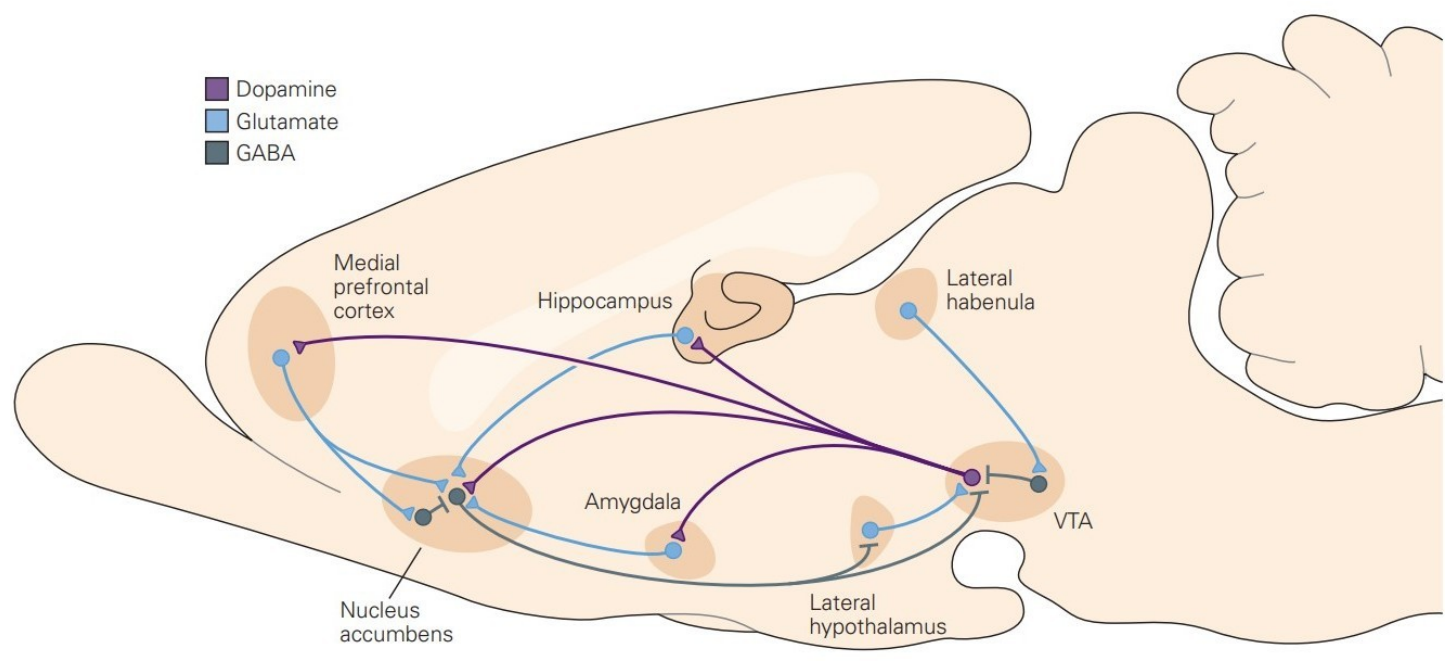
\includegraphics[width=\linewidth]{media/8-ratbrain.png}
	\caption{Diagram showing the VTA's projections in a rat's brain. When the VTA activates, dopaminergic neurons (in purple) form excitatory projections into different parts of the brain (hippocampus, amygdala, NAc...) producing the emotion of reward.}
	\label{ratbrain}
\end{figure}

However, this explanation on addiction isn't still completely solid. Identifying dopamine as a \enquote{pleasure neurotransmitter} is wrong. Sometimes dopamine signals negative responses, and more recent studies have associated its liberation to an \enquote{error in prediction}.

Furthermore, the activation of dopaminergic neurons is only one component of all neural processes that occur during the reward emotion. Rats lacking dopamine still show hedonic behavior towards sugar and cocaine, which indicates that this neurotransmitter isn't the only relevant factor.

Even worse, the pattern of doing something repeatedly even in self-detriment can be applied to behaviors such as gambling, food and sex. These are very complex topics to study, as it's impossible to construct a human model of a rat with shopping addiction. Even in rodents it's hard to find deterministic patterns: groups of rats won't develop addiction to cocaine in the same proportions when they are totally isolated and when they are inside \enquote{enriched environments} with partners, polyethylene tubes and balls.

What parallels can be drawn between a rat's behavior and a human's? How is addiction manifested at a neural scale and how is it really related to drugs? We again find the mantra we've repeated again and again during every neuroscience investigation: we don't know. Having no universal statements to make, we are forced to analyse the specific effects of LSD.

\newpage

\subsection{Pharmacology of LSD.}

Lysergic acid's diethylamide is a semisynthetic drug derived from lysergic acid extracted from ergot. It has four stereoisomers, that is, four structurally sister compounds: l- and d- LSD and l- and d- iso-LSD. Only d-LSD is psychoactive, and it's the one we refer to when saying \enquote{LSD}. It's soluble in water and melts at 83$^\circ$C, and because of its sensitivity to light, temperature and humidity it is usually stored as a tartrate salt. Due to its high bioavailability, the most common administration route is the oral route. Originally it was done through ampoules, but it became popular to soak blotting paper or sugar cubes with it and place those on the tongue. Different doses of LSD produce different effects.

In an individual between 50 and 70 kg of body weight, the minimum recognisable dose is 25 $\mu$g, and produces some cognitive changes. The standard dose lies between 70 and 100 $\mu$g, and has effects lasting from 6 to 10 hours, including visionary ones. From 300 $\mu$g up begin the high doses, with very intense effects lasting longer than 10 hours.

The average lethal dose in different animals lies between 0.3 and 16.5 mg / kg, being 1 mg / kg in monkeys. The lethal dose for humans is unknown, as there are no recorded deaths by LSD. There's a case of eight individuals who mistaked LSD for cocaine and took a very large dose. They were measured to have 1-7 mg of the substance for each 100 mL of blood. They suffered from comatose states, hyperthermia, vomits, gastric bleeding and trouble breathing, but with hospitalary assistance, they all survived without lasting consequences. It's then safe to say that LSD's safety margin is extraordinarily high.

LSD presents a very high tolerance. After doses ranging from 5 to 100 micrograms administered during 3 to 6 days, volunteers develop a strong tolerance. This disappears after about 4 days of no use. Apart from that, there is a general consensus on the fact that LSD isn't addictive, that is, it doesn't produce the compulsive seek behavior for new doses.

It's clear this substance has exceptional properties, however, it being pharmacologically safe doesn't imply that it's general use is safe. There are documented cases of self harm and suicide under the effects of this drug, although the numbers are small. More details on this behalf are given on section \ref{now-history}.

\newpage

\subsection{LSD's effects.}

A standard dose of LSD significantly alters the state of consciousness, with a tendency to euphoria, that is, a very intense state of happiness and well-being; a boost in introspection abilities and the stimulation of primary Freudian processes, in other words, instinctive desires are unleashed, inhibiting the influence of ego and society upon the individual. The most characteristic effect are the alterations in perception like illusions, visions, pseudohallucinations, synesthesias --- the capability to cross senses --- and alterations on thought and time perception. A special mention is required for the changes it makes on self-perception and the function of the ego. LSD (specially in higher dosages) blurs the border that separates the \textit{I} from the rest of the world, a phenomenon known as \enquote{ego death} or \enquote{dissolution}.

The unmatched potency of LSD is a double-edged sword, because just as its capable of providing a good experience and positive psychological effects in the long term, it can also induce traumatic experiences (colloquially known as \enquote{bad trips}) with negative effects like mood swings and, sometimes, retrospective scenes which can be harmful. It's difficult to study LSD's effects on thought, as we can't get into anyone's mind and the standard dose is already enough to hinder communication during the experiments. It can be stated that LSD reduces skill in tests requiring attention and focus, psychomotor and arithmetic skills, visual memory and temporal perception --- time intervals tend to be overestimated. Learning processes aren't affected. Some interpretations say that intellectual functions suffer a setback to an earlier stage of development. No faculty is known to be harmed in a chronic way by the use of LSD. In many people it causes dizziness and internal agitation.

\subsection{Mechanism of action: the serotoninergic system.}

Serotonin (also called 5-hidroxytryptamine or 5-HT) is a neurotransmitter made from tryptophan in very few neurons (counted in the thousands). These neurons are found mainly in the mid-brain's \textit{raphe nuclei}, and they project their connections to regions like the hippocampus, the cerebral cortex, the NAc and dopaminergic nuclei like the VTA, among others (Figure \ref{pathways}). The connection between the raphe nuclei and the \textit{locus coeruleus} (LC) is quite important, as this region takes charge of the liberation of noradrenaline and has connections to the cerebellum, the thalamus, the hypothalamus, the cortex and the hippocampus.

It's obvious that, even though they are few in number, the abundant outward connections from the serotoninergic neurons (up to 500.000 per neuron) make 5-HT a crucial neurotransmitter in very different processes, like the regulation of mood, body temperature and even the gastrointestinal tract. Deficiencies in levels of serotonin are associated to depressive disorders, which are treated through many forms of psychotherapy and antidepressant pharmaceuticals (normally, selective serotonin reuptake inhibitors or SSRIs, like fluoxetine and sertraline).

The serotoninergic system is also related to the filtering of information in the brain. Not every stimulus is equally relevant, and some --- like the foliage's sound --- are continuous and repetitive, so they don't deserve constant attention. The brain has a limited capacity for processing data, so it automatically discards this information to leave space for more important one, avoiding a sensory overload. An alteration in this screening could explain LSD's stimulating and hallucinogenic effects.

LSD's molecular structure is similar to that of serotonin, which allows it to join to some of its receptors, although with less strength than actual serotonin (it is what's known as a \textit{partial agonist}). This interaction alters the serotonin system's behavior, although it's not exactly known how. Neurons from the serotonin system count with up to 14 different receptors (and a 15th one is theorized), some of them being inhibitory and others excitatory, but most of them metabotropic (that is, they don't directly control the channel's opening and closing, but instead modulate the neuron's activity through second messengers). These receptors are denoted like \enquote{5-HT$_{\textrm{XY}}$} (Y serotonin receptor of the X class).

More specifically, it acts as a partial agonist on receptors 5-HT$_{\textrm{1A}}$, 5-HT$_{\textrm{2A}}$ and 5-HT$_{\textrm{2C}}$, but also on other neurotransmitters' receptors like the dopaminergic D$_2$ receptor and the adrenergic $\alpha_2$ receptor. A side effect of stimulating 5-HT$_{\textrm{2A}}$ receptors is the activation of glutamatergic transmission in the frontal cortex. This is a key pattern shared by LSD and other serotoninergic hallucinogens, and it is believed that this activation could cause a disturbance in the sensory and cognitive gating systems. Tolerance could occur due to a decrease in 5-HT$_{\textrm{2A}}$ receptor density.

\begin{figure}[H]
	\centering
	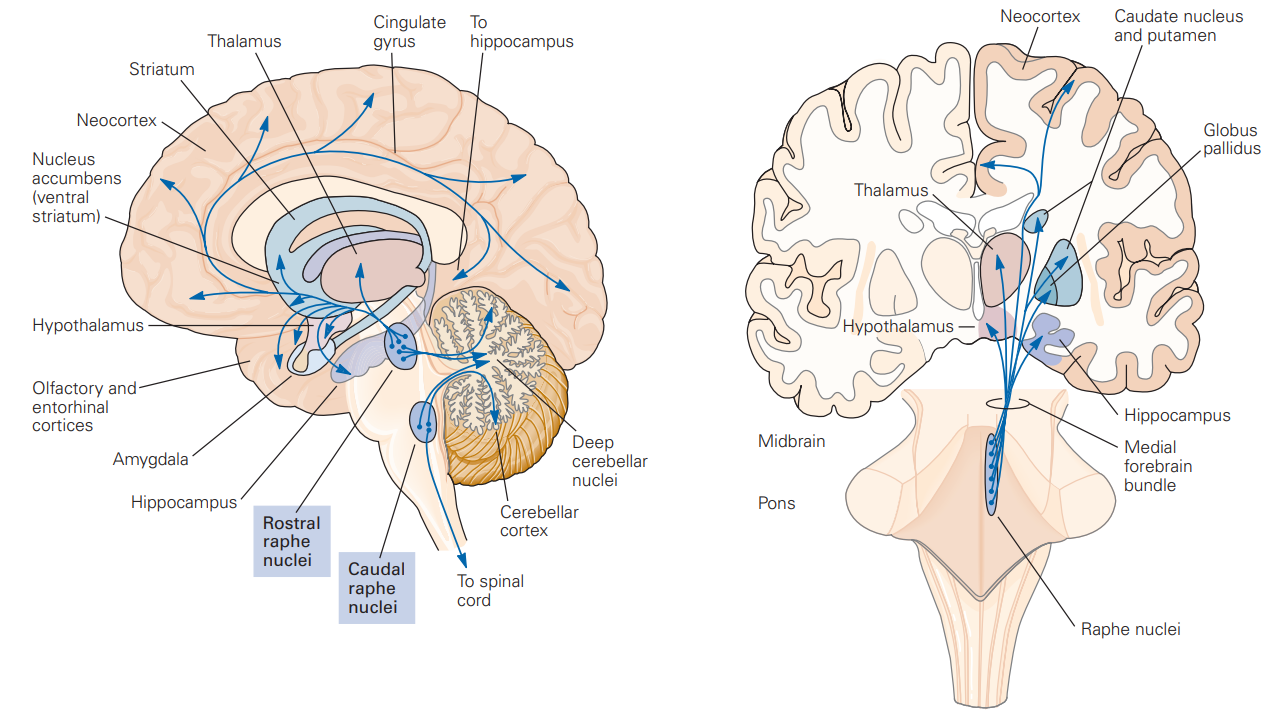
\includegraphics[width=\linewidth]{media/9-pathways.png}
	\caption{Encephalic serotoninergic pathways. Serotoninergic neurons born in the raphe nuclei project outwards to many encephalic regions.}
	\label{pathways}
\end{figure}

\newpage
